\chapter{Diseño}


\section{Introducción}

En el desarrollo de software, es fundamental para los desarrolladores tener una idea clara sobre el funcionamiento del programa a realizar para ello se basan en herramientas que les permiten realizar el análisis de requerimientos para complacer las necesidades del cliente, a continuación veremos el proceso de análisis de dichos requerimientos para nuestro problema en particular

\section{Requerimientos}
Los principales requeremientos se presentaran acontinuacion en las siguientes tablas

\begin{table}[th!]
	\centering
	\caption{REQ EXPANDIR NEGOCIO}
	\label{my-label}
	\begin{tabular}{|l|l|l|}
		\hline
		ID del requisito                                                             & \multicolumn{2}{c|}{REQ EN}                                                                                                                                                                \\ \hline
		Versión                                                                      & \multicolumn{2}{c|}{1}                                                                                                                                                                     \\ \hline
		Autores                                                                      & \multicolumn{2}{c|}{Sebastian Bohorquez, Johan Perez, Juan Cubillos}                                                                                                                       \\ \hline
		Descripción                                                                  & \multicolumn{2}{l|}{\begin{tabular}[c]{@{}l@{}}Las empresas PYME desean ampliar las ventas de sus\\ negocios  mediante la venta de sus productos a \\ través de plataformas web\end{tabular}} \\ \hline
		Precondicion                                                                 & \multicolumn{2}{l|}{}                                                                                                                                                                      \\ \hline
		\multirow{2}{*}{\begin{tabular}[c]{@{}l@{}}Secuencia \\ normal\end{tabular}} & Paso                         & Acción                                                                                                                                                      \\ \cline{2-3} 
		& 1                            & \begin{tabular}[c]{@{}l@{}}Crear una plataforma web para las empresas\\ PYME en la que puedan publicitar sus productos\end{tabular}                        \\ \hline
		Postcondicion                                                                & \multicolumn{2}{l|}{REQ REL Y REQ PP}                                                                                                                                                      \\ \hline
		Excepciones                                                                  & Paso                         & Acción                                                                                                                                                      \\ \hline
		& 1                            & Otros países                                                                                                                                                \\ \hline
		Importancia                                                                  & \multicolumn{2}{l|}{Primordial}                                                                                                                                                            \\ \hline
		Urgencia                                                                     & \multicolumn{2}{l|}{Primordial}                                                                                                                                                            \\ \hline
		Comentarios                                                                  & \multicolumn{2}{l|}{}                                                                                                                                                                      \\ \hline
	\end{tabular}
\end{table}

\newpage
\begin{table}[th!]
	\centering
	\caption{REQ PUBLICITAR PRODUCTO}
	\label{my-label2}
	\begin{tabular}{|l|l|l|}
		\hline
		ID del requisito                                                             & \multicolumn{2}{l|}{REQ PP}                                                                                                                                                                                       \\ \hline
		Versión                                                                      & \multicolumn{2}{c|}{1}                                                                                                                                                                                            \\ \hline
		Autores                                                                      & \multicolumn{2}{c|}{Sebastian Bohorquez, Johan Perez, Juan Cubillos}                                                                                                                                              \\ \hline
		Descripción                                                                  & \multicolumn{2}{l|}{\begin{tabular}[c]{@{}l@{}}Mediante el uso de una plataforma web, las empresas PYME\\ podrán publicitar sus productos mostrando sus características y  \\el inventario del mismo.\end{tabular}} \\ \hline
		Precondicion                                                                 & \multicolumn{2}{l|}{REQ EN}                                                                                                                                                                                       \\ \hline
		\multirow{6}{*}{\begin{tabular}[c]{@{}l@{}}Secuencia\\  normal\end{tabular}} & Paso                                                                        & Acción                                                                                                                              \\ \cline{2-3} 
		& 1                                                                           & Establecer id del producto                                                                                                          \\ \cline{2-3} 
		& 2                                                                           & Subir imagen del producto a publicar                                                                                                \\ \cline{2-3} 
		& 3                                                                           & Indicar las características del producto ya seleccionado                                                                       \\ \cline{2-3} 
		& 4                                                                           & Indicar el inventario del producto                                                                                                  \\ \cline{2-3} 
		& 5                                                                           & Publicar Producto                                                                                                                   \\ \hline
		Postcondicion                                                                & \multicolumn{2}{l|}{}                                                                                                                                                                                             \\ \hline
		\multirow{6}{*}{Excepciones}                                                 & Paso                                                                        & Acción                                                                                                                              \\ \cline{2-3} 
		&                                                                             & El producto agregado ya existe                                                                                                      \\ \cline{2-3} 
		& 1                                                                           & Modificar publicación del producto                                                                                                  \\ \cline{2-3} 
		& 2                                                                           & Cambiar características                                                                                                             \\ \cline{2-3} 
		& 3                                                                           & Modificar inventario                                                                                                                \\ \cline{2-3} 
		& 4                                                                           & Publicar el producto con los nuevos cambios                                                                                         \\ \hline
		Importancia                                                                  & \multicolumn{2}{l|}{Primordial}                                                                                                                                                                                   \\ \hline
		Urgencia                                                                     & \multicolumn{2}{l|}{Primordial}                                                                                                                                                                                   \\ \hline
		Comentarios                                                                  & \multicolumn{2}{l|}{}                                                                                                                                                                                             \\ \hline
	\end{tabular}
\end{table}
\newpage
\begin{table}[th!]
	
	\caption{REQ RECAUDO EN LINEA}
	\label{my-label3}
	\begin{tabular}{|l|l|l|}
		\hline
		ID del requisito                                                             & \multicolumn{2}{c|}{REQ REL}                                                                                                                                                                                                                                         \\ \hline
		Versión                                                                      & \multicolumn{2}{c|}{1}                                                                                                                                                                                                                                               \\ \hline
		Autores                                                                      & \multicolumn{2}{c|}{Sebastian Bohorquez, Johan Perez, Juan Cubillos}                                                                                                                                                                                                 \\ \hline
		Descripción                                                                  & \multicolumn{2}{l|}{\begin{tabular}[c]{@{}l@{}}Una vez publicado el producto se podrá proceder a la compra \\del mismo, teniendo en cuenta la verificación del medio de \\pago y se procederá a pedir los datos del usuario para el \\posterior envió\end{tabular}} \\ \hline
		Precondicion                                                                 & \multicolumn{2}{l|}{REQ EN}                                                                                                                                                                                                                                          \\ \hline
		\multirow{8}{*}{\begin{tabular}[c]{@{}l@{}}Secuencia \\ normal\end{tabular}} & Paso                                                                   & Acción                                                                                                                                                                                      \\ \cline{2-3} 
		& 1                                                                      & Seleccionar un producto                                                                                                                                                                     \\ \cline{2-3} 
		& 2                                                                      & Indicar el método de pago para la compra del producto                                                                                                                                       \\ \cline{2-3} 
		& 3                                                                      & \begin{tabular}[c]{@{}l@{}}Verificar el medio de pago ingresado por el usuario \\ (tarjeta débito o crédito)\end{tabular}                                                                   \\ \cline{2-3} 
		& 4                                                                      & Ingresar datos del usuario para el envió del producto                                                                                                                                       \\ \cline{2-3} 
		& 5                                                                      & Confirmar compra del producto y generar recibo.                                                                                                                                             \\ \cline{2-3} 
		& 6                                                                      & Recibir notificación de pago                                                                                                                                                                \\ \cline{2-3} 
		& 7                                                                      & Despacho del producto                                                                                                                                                                       \\ \hline
		Postcondicion                                                                & \multicolumn{2}{l|}{}                                                                                                                                                                                                                                                \\ \hline
		\multirow{6}{*}{Excepciones}                                                 & Paso                                                                   & Acción                                                                                                                                                                                      \\ \cline{2-3} 
		&                                                                        & El método de pago es incorrecto                                                                                                                                                             \\ \cline{2-3} 
		& 1                                                                      & Cambiar método de pago                                                                                                                                                                      \\ \cline{2-3} 
		&                                                                        & El producto no se encuentra disponible                                                                                                                                                      \\ \cline{2-3} 
		& 1                                                                      & Cancelar compra                                                                                                                                                                             \\ \cline{2-3} 
		& 2                                                                      & Seleccionar otro producto                                                                                                                                                                   \\ \hline
		Importancia                                                                  & \multicolumn{2}{l|}{Primordial}                                                                                                                                                                                                                                      \\ \hline
		Urgencia                                                                     & \multicolumn{2}{l|}{Primordial}                                                                                                                                                                                                                                      \\ \hline
		Comentarios                                                                  & \multicolumn{2}{l|}{}                                                                                                                                                                                                                                                \\ \hline
	\end{tabular}
\end{table}
\newpage
\subsection{Casos de Uso}

Un diagrama de casos de uso nos sirve para observar el “QUE” del sistema, mostrando procesos que deberán ser resueltos según las necesidades (requerimientos) del cliente, en este caso el cliente requiere que el sistema PYME pueda expandir su negocio así ampliando el mercado del mismo, en el siguiente diagrama se plantea una solución al cliente enfocado en dicho sistema teniendo en cuenta tanto sus requerimientos como sus actores y qué papel desempeña en el sistema.


\begin{figure}[th!]
	\centering
	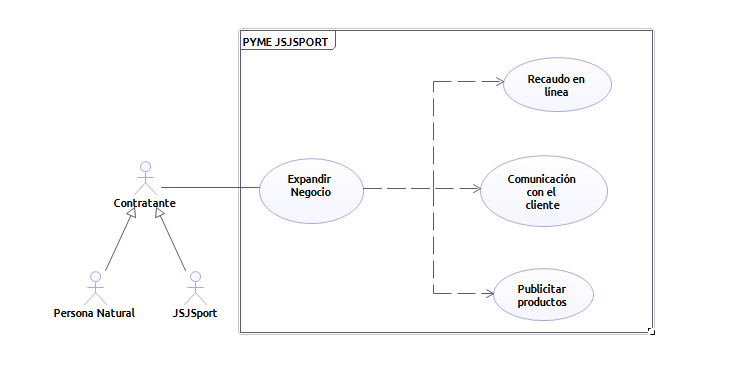
\includegraphics[width=0.7\linewidth]{arquitectura/imagenes/casosDeUso}
	\caption{Diagrama de  casos de Uso}
\end{figure}

El proceso de expandir el negocio, como  se puede observar en el diagrama, incluye dos procesos importantes, el primero de ellos es que el sistema pueda publicitar productos, en otras palabras,  brindar al cliente una plataforma web donde pueda exponer sus productos hacia al público deseado, teniendo en cuenta los aspectos como su inventario, apoyándose con una base de datos.

El proceso de recaudo en línea, consiste en todo lo relacionado con la compra y venta del producto que se ofrecen en la plataforma web anteriormente generada, y verifica que el medio de pago ingresado por el usuario sea válido, una vez se compruebe el paso anterior se procederá a la confirmación de la compra, generando un comprobante de pago para la empresa y para el usuario para finalmente  proceder a pedirle al usuario que ingrese los datos del domicilio.


\newpage


\section{Escenarios}

\subsection{Diagrma de secuencia}

\subsection{Diagrma de comunicación}

\newpage

\section{Clases}

\newpage

\section{Componentes}

\newpage

\section{Nodos}

\newpage

\section{Sistemas}

\newpage

\section{Actividades}

\newpage

\section{Estados}

\newpage






